\documentclass[12pt,a4paper]{article}
\usepackage[utf8]{inputenc}
\usepackage{amsmath}
\usepackage{textcomp}

\usepackage{geometry}
\geometry{a4paper,left=25mm,right=25mm, top=2cm, bottom=2cm} 

\usepackage{verbatim}

 \usepackage{mathptmx}
 \usepackage[scaled=.90]{helvet}
 \usepackage{courier}

\usepackage[utf8]{inputenc}

\usepackage{listings}
\usepackage{color}

\usepackage{graphicx}
 
\definecolor{dkgreen}{rgb}{0,0.6,0}
\definecolor{gray}{rgb}{0.5,0.5,0.5}
\definecolor{mauve}{rgb}{0.58,0,0.82}

\pagestyle{empty}
\lstset{numbers=left,language=C++}
\lstset{showstringspaces=false,
basicstyle=\ttfamily\footnotesize,
breaklines=true,
tabsize=3,
commentstyle=\color{dkgreen},       % comment style
}

%keine einrückungen bei absatz
\parindent 0pt

\begin{document}
\title{Übung 6}
\author{Bernhard Selymes, Reinhard Penn}
\date{Dezember 2012}

\normalsize

%Pfad zu c++ Dateien
\newcommand{\CodePath}{../MusicPlayer/MusicPlayer/}

%Beginn des Dokuments
\section{Organisatorisches}

\subsection{Team}
	\begin {itemize} 
		\item Reinhard Penn, s1110306019 
		\item Bernhard Selymes, s1110306024
	\end {itemize}

\subsection{Aufteilung}
	\begin {itemize} 
		\item Reinhard Penn
			\begin {itemize}
				\item Planung
				\item Klassendiagramm
				\item Implementierung der Klassen MusicFactory, MusicComponent, Song, Album, MusicCollection
				\item Testen aller Klassen
			\end {itemize}
		\item Bernhard Selymes
			\begin {itemize}
				\item Planung
				\item Klassendiagramm
				\item Implementierung der Klassen Visitor, TimeVisitor, SearchVisitor, PlayVisitor, MusicPlayer
				\item Dokumentation		
			\end {itemize}
	\end {itemize}


\subsection{Zeitaufwand}
	\begin {itemize}
		\item geschätzte Mh: 15
		\item tatsächlich: Reinhard (10h), Bernhard  (10h)
	\end {itemize}


\section{Systemspezifikation}
Es soll eine Software für die Verwaltung von Musikmedien entworfen werden. Ein Musikmedium kann ein Lied, ein Album oder eine Musikkollektion sein. Ein Album besteht aus Liedern, eine Kollektion kann aus allen Arten von Musikmedien bestehen. Für alle Medien wirde der Name gespeichert, für das Album zusätzlich der Interpret, für das Lied zusätzlich Interpret, Album Spieldauer in Minuten und Sekunden. Mit dem Musik Player kann man Musikmedien hinzufügen und entfernen, diese wiedergeben (via std::cout), die Spieldauer einzelner oder aller Musikmedien herausfinden und nach Musikmedien suchen.
\\


\newpage
\section {Systementwurf}

\subsection {Klassendiagramm}

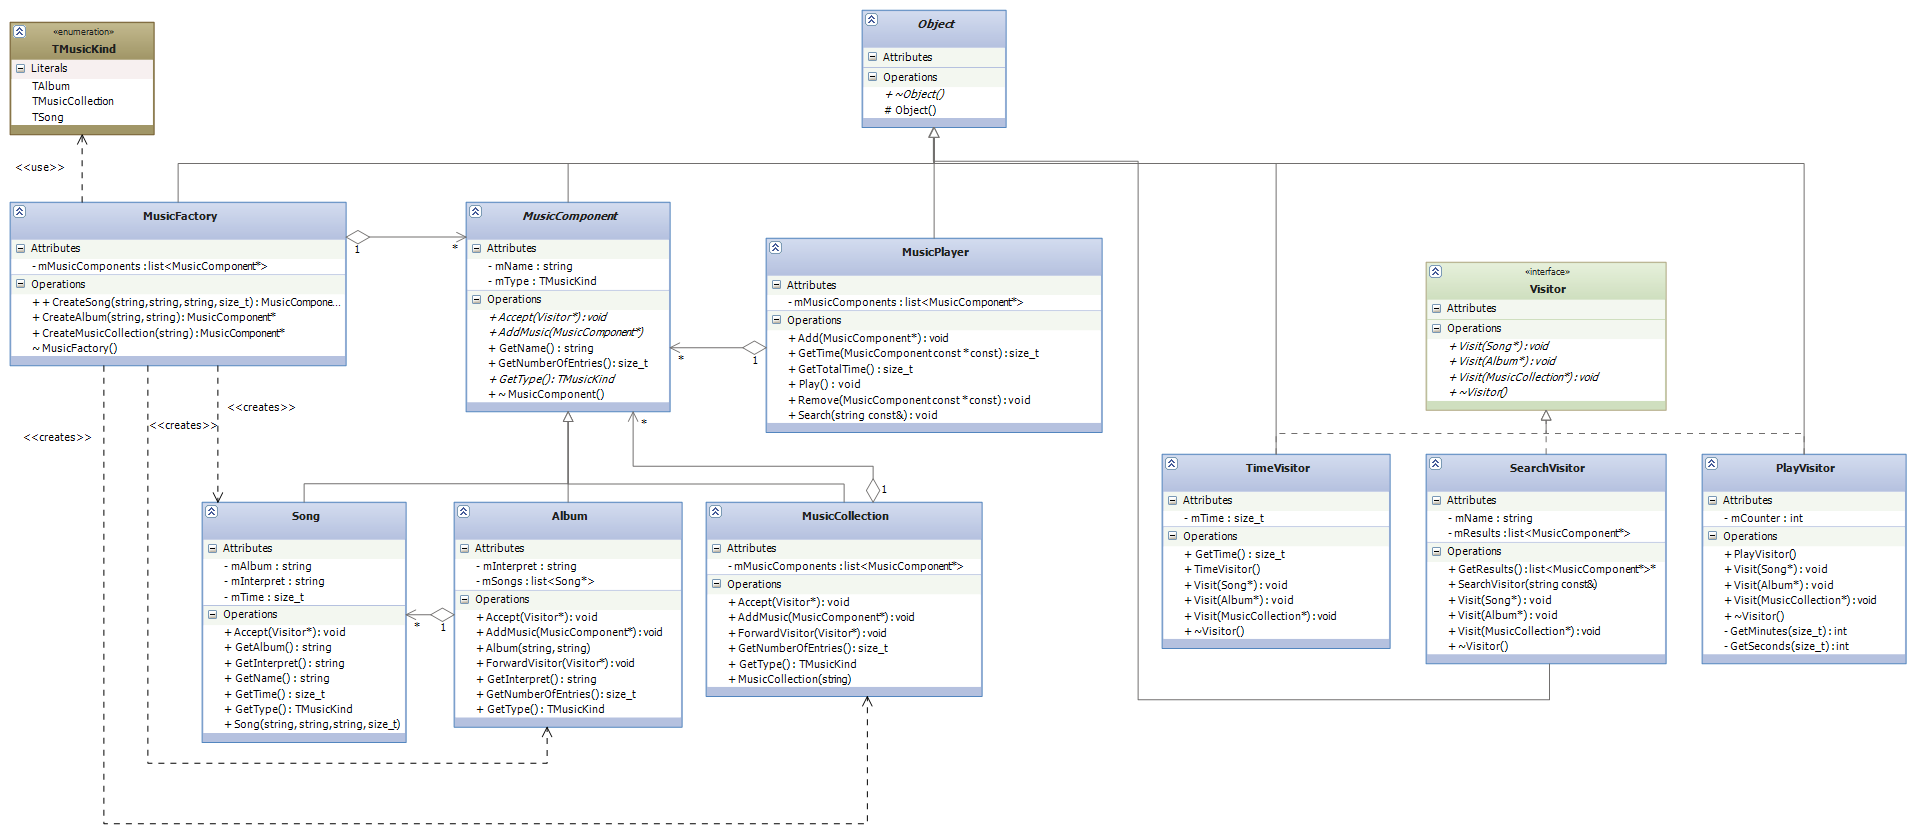
\includegraphics[angle=90,scale=0.5] {../Klassendiagramm.png}

\newpage
\subsection {Komponentenübersicht}
\begin {itemize} 
	\item Klasse "Object":
	\newline
	Basis aller Basisklassen.
	
	\item Enumeration "MusicKind":
	\newline
	Definiert die verschiedenen Arten von Musikmedien.

	\item Klasse "MusicFactory":
	\newline
	Zuständig für die Erzeugung der Objekte.

	\item Klasse "MusicComponent":
	\newline
	Basisklasse für Musikmedien.

	\item Klasse "Song":
	\newline
	Abgeleitet von MusicComponent.
	
	\item Klasse "Album":
	\newline
	Abgeleitet von MusicComponent.

	\item Klasse "MusicCollection":
	\newline
	Abgeleitet von MusicComponent.
	
	\item Interface "Visitor":
	\newline	
	Abstrakte Basisklasse für Visitors.
	
	\item Klasse "TimeVisitor":
	\newline
	Abgeleitet von Visitor. Visitor für Spieldauer.
	
	\item Klasse "SearchVisitor":
	\newline
	Abgeleitet von Visitor. Visitor für die Suche nach Medien.
	
	\item Klasse "PlayVisitor":
	\newline
	Abgeleitet von Visitor. Visitor für das Abspielen von Medien.

	\item Klasse "MusicPlayer":
	\newline
	Klasse die die Medien verwaltet und alles mögliche mit ihnen machen kann.
		
\end {itemize}

\newpage
\section {Komponentenentwurf}
\subsection {Klasse "Object"}
Abstrakte Basisklasse aller Klassen. Von ihr werden alle anderen Klassen abgeleitet. Beinhaltet einen virtuellen Destruktor.

\subsection {Enumeration "TMusicKind"}
\begin {itemize}
	\item TSong
	\item TAlbum
	\item TMusicCollection	
\end {itemize}


\subsection {Klasse "MusicFactory"}
Kann Musikmedien dynamisch anlegen und wieder freigeben. In einer Liste werden die Referenzen auf die Objekte gespeichert. Die Methoden legen die Objekte je nach Medientyp mit den übergebenen Parametern an und fügen sie der Liste hinzu. Die Factory darf nur nach dem Musikplayer gelöscht werden, es kann nicht überprüft werden ob die Referenzen auf Objekte noch im Musicplayer gespeichert sind, weil keine Verbindung zwischen den beiden Klassen besteht.
\\

\subsection {Klasse "MusicComponent"}
Bietet die Schnittstellen für die Methoden "Accept", "GetType", "GetNumberOfEntries" und "AddMusic", "GetName" wird implementiert. Hat zwei Member die Namen und Type speichern.
\\

\textbf {Methode "GetName": } 
\newline
Schnittstelle:
\newline
Rückgabetyp: string
\newline
Get Funktion.
\\

\subsection {Klasse "Song"}
Hat Member die den Namen des Albums und des Interpreten und die Spieldauer in Sekunden speichert. Wir haben uns für Sekunden entschieden, weil die Übergabe leichter ist (keine extra Struktur), das Addieren von mehreren Zeiten umständlich wäre und die Sekunden für die Ausgabe und weitere Verwendung leicht umgerechnet werden können. Hat einige Getter Funktionen.
\\

\textbf {Methode "Accept": } 
\newline
Schnittstelle: 
\newline
Parameter: Visitor*
\newline
Rückgabetyp: void
\newline
Ruft die Funktion Visit vom übergebenen Visitor mit sich selbst auf.
\\

\subsection {Klasse "Album"}
Hat Member die den Namen des Interpreten und eine Liste die die Lieder des Albums speichert. Hat einige Getter Funktionen.
\\

\textbf {Methode "Accept": } 
\newline
Schnittstelle: 
\newline
Parameter: Visitor*
\newline
Rückgabetyp: void
\newline
Ruft die Funktion Visit vom übergebenen Visitor mit sich selbst auf.
\\

\textbf {Methode "ForwardVisitor": } 
\newline
Schnittstelle:
\newline
Parameter: Visitor*
\newline
Rückgabetyp: void
\newline
Ruft für alle Lieder die Funktion "Accept" mit dem Visitor auf.
\\

\textbf {Methode "GetTime": } 
\newline
Schnittstelle:
\newline
Rückgabetyp: void
\newline
Ruft für alle Lieder die Methode "Accept" mit dem Visitor auf.
\\

\textbf {Methode "AddMusic": } 
\newline
Schnittstelle:
\newline
Parameter: MusicComponent*
\newline
Rückgabetyp: void
\newline
Fügt ein Lied (und nur ein Lied) zur Liste hinzu.
\\

\subsection {Klasse "MusicCollection"}
Hat eine Liste die alle Musikmedien, die in der Kollektion enthalten sind.
\\

\textbf {Methode "Accept": } 
\newline
Schnittstelle: 
\newline
Parameter: Visitor*
\newline
Rückgabetyp: void
\newline
Ruft die Funktion Visit vom übergebenen Visitor mit sich selbst auf.
\\

\textbf {Methode "ForwardVisitor": } 
\newline
Schnittstelle:
\newline
Rückgabetyp: void
\newline
Ruft für alle Musikmedien die Methode "Accept" mit dem Visitor auf.
\\

\textbf {Methode "GetNumberOfEntries": } 
\newline
Schnittstelle:
\newline
Rückgabetyp: size\_t
\newline
Ruft für alle Musikmedien die Funktion "GetNumberOfEntries" auf und addiert sie.
\\

\subsection {Interface "Visitor"}
Definiert die Schnittstellen der Methoden.
\\

\textbf {Methoden "Visit": } 
\newline
Schnittstelle: 
\newline
Parameter: Song* oder Album* oder MusicCollection*
\newline
Rückgabetyp: void
\newline
Pure virtual function.
\\

\subsection {Klasse "TimeVisitor"}
Hat einen Member der die gesamte Dauer speichert.
\\

\textbf {Methode "Visit": } 
\newline
Schnittstelle: 
\newline
Parameter: Song*
\newline
Rückgabetyp: void
\newline
Addiert zum Gesamtdauermember die Dauer vom Lied.
\\

\textbf {Methode "Visit": } 
\newline
Schnittstelle: 
\newline
Parameter: Album*
\newline
Rückgabetyp: void
\newline
Ruft die Funktion "ForwardVisitor" vom Album mit sich selbst (Visitor) auf.
\\

\textbf {Methode "Visit": } 
\newline
Schnittstelle: 
\newline
Parameter: MusicCollection*
\newline
Rückgabetyp: void
\newline
Ruft die Funktion "ForwardVisitor" von der Kollektion mit sich selbst (Visitor) auf.
\\

\subsection {Klasse "SearchVisitor"}
Hat einen Member der den gesuchten Namen speichert und eine Liste die Referenzen zu den gefundenen Objekten speichert.
\\

\textbf {Methode "Visit": } 
\newline
Schnittstelle: 
\newline
Parameter: Song*
\newline
Rückgabetyp: void
\newline
Schaut ob der gesuchte Name Teil des Namens vom Lied ist und speichert in ggf. in der Liste.
\\

\textbf {Methode "Visit": } 
\newline
Schnittstelle: 
\newline
Parameter: Album*
\newline
Rückgabetyp: void
\newline
Ruft die Funktion "ForwardVisitor" vom Album mit sich selbst (Visitor) auf.
\\

\textbf {Methode "Visit": } 
\newline
Schnittstelle: 
\newline
Parameter: MusicCollection*
\newline
Rückgabetyp: void
\newline
Ruft die Funktion "ForwardVisitor" von der Kollektion mit sich selbst (Visitor) auf.
\\

\subsection {Klasse "PlayVisitor"}
Hat einen Zähler der die Nummer der Lieder bestimmt.
\\

\textbf {Methode "Visit": } 
\newline
Schnittstelle: 
\newline
Parameter: Song*
\newline
Rückgabetyp: void
\newline
Gibt die Daten des Liedes formatiert auf der Konsole aus und erhöht den Zähler.
\\

\textbf {Methode "Visit": } 
\newline
Schnittstelle: 
\newline
Parameter: Album*
\newline
Rückgabetyp: void
\newline
Legt einen TimeVisitor an. Dieser wird vom Album accepted. Die Informationen des Albums werden auf der Konsole ausgegeben. Danach wird der Visitor den Elementen im Album weitergegeben.
\\

\textbf {Methode "Visit": } 
\newline
Schnittstelle: 
\newline
Parameter: MusicCollection*
\newline
Rückgabetyp: void
\newline
Legt einen TimeVisitor an. Dieser wird von der Kollektion akkzeptiert. Die Informationen der Kollektion werden auf der Konsole ausgegeben. Danach wird der Visitor den Elementen in der Kollektion weitergegeben.
\\

\subsection {Klasse "MusicPlayer"}
Hat einen Liste mit Musik-Medien.
\\

\textbf {Methode "GetTime": } 
\newline
Schnittstelle: 
\newline
Parameter: MusicComponent* const
\newline
Rückgabetyp: size\_t
\newline
Prüft zuerst ob das Element überhaupt vorhanden ist. Dann wird via eines TimeVisitors die Dauer des Elements ermittelt.
\\

\textbf {Methode "GetTotalTime": } 
\newline
Schnittstelle: 
\newline
Rückgabetyp: size\_t
\newline
Via eines TimeVisitors die Dauer aller Elemente ermittelt.
\\

\textbf {Methode "Play": } 
\newline
Schnittstelle: 
\newline
Rückgabetyp: void
\newline
Via eines PlayVisitors wird die gesamte Abspielliste ausgegeben.
\\

\textbf {Methode "Search": } 
\newline
Schnittstelle: 
\newline
Parameter: string const\&
\newline
Rückgabetyp: void
\newline
Via eines SearchVisitors wird der Name überall gesucht. Der Name der gefundenen Elemente wird danach ausgegeben.
\\

\newpage
\section {Source Code}

\lstinputlisting[language=C++]{\CodePath Object.h}
\lstinputlisting[language=C++]{\CodePath Object.cpp}
\newpage

\lstinputlisting[language=C++]{\CodePath TMusicKind.h}
\newpage

\lstinputlisting[language=C++]{\CodePath MusicFactory.h}
\newpage
\lstinputlisting[language=C++]{\CodePath MusicFactory.cpp}
\newpage

\lstinputlisting[language=C++]{\CodePath MusicComponent.h}
\newpage
\lstinputlisting[language=C++]{\CodePath MusicComponent.cpp}
\newpage

\lstinputlisting[language=C++]{\CodePath Song.h}
\newpage
\lstinputlisting[language=C++]{\CodePath Song.cpp}
\newpage

\lstinputlisting[language=C++]{\CodePath Album.h}
\newpage
\lstinputlisting[language=C++]{\CodePath Album.cpp}
\newpage

\lstinputlisting[language=C++]{\CodePath MusicCollection.h}
\newpage
\lstinputlisting[language=C++]{\CodePath MusicCollection.cpp}
\newpage

\lstinputlisting[language=C++]{\CodePath Visitor.h}
\newpage

\lstinputlisting[language=C++]{\CodePath TimeVisitor.h}
\newpage
\lstinputlisting[language=C++]{\CodePath TimeVisitor.cpp}
\newpage

\lstinputlisting[language=C++]{\CodePath SearchVisitor.h}
\newpage
\lstinputlisting[language=C++]{\CodePath SearchVisitor.cpp}
\newpage

\lstinputlisting[language=C++]{\CodePath PlayVisitor.h}
\newpage
\lstinputlisting[language=C++]{\CodePath PlayVisitor.cpp}
\newpage

\lstinputlisting[language=C++]{\CodePath MusicPlayer.h}
\newpage
\lstinputlisting[language=C++]{\CodePath MusicPlayer.cpp}
\newpage

\lstinputlisting[language=C++]{\CodePath main.cpp}
\newpage

\section {Testausgaben} 

\begin {verbatim}
Testcase0: Empty testcase with NULL pointer.
Add: error in MusicPlayer::Add(): no valid pointer
 ...done
GetTime: error in MusicPlayer::GetTime(): no valid pointer
 ...done
GetTotalTime:  ...done
Play:
 ...done
Remove: error in MusicPlayer::Remove(): no valid pointer
 ...done
Search: error in MusicPlayer::Search(): no valid name
 ...done
Delete MusicPlayer:  ...done
Delete MusicFactory:  ...done


Testcase1: Normal testcase with valid objects.
Create Objects:  ...done
Put Albums together:  ...done
Put an album into an album: Error in Album::AddMusic: 
Tried to add a wrong object type to the song list
 ...done
Put Collection together:  ...done
Put a collection into itself: Error in MusicCollection::AddMusic: 
no valid pointer
 ...done
Add stuff to the player:  ...done
GetTime: error in MusicPlayer::GetTime(): component doesnt exist in list
0 seconds ...done
GetTotalTime: 1359 seconds in player ...done
Play:
1. Staring At The Sun << 02:12 << The Offspring
Collection: MyPlayList (3 Song(s))  << 10:51
Album: Americana (2 Song(s))  << 06:08
2. Staring At The Sun << 02:12 << The Offspring
3. Have You Ever << 03:56 << The Offspring
4. Psychosocial << 04:43 << Slipknot
Album: Conspiracy Of One (1 Song(s))  << 03:28
5. Living In Chaos << 03:28 << The Offspring
Album: Americana (2 Song(s))  << 06:08
6. Staring At The Sun << 02:12 << The Offspring
7. Have You Ever << 03:56 << The Offspring
 ...done
Search: found medias: (search for "in")
Staring At The Sun
Staring At The Sun
Living In Chaos
Staring At The Sun
 ...done
Remove:  ...done
Play after remove:
1. Staring At The Sun << 02:12 << The Offspring
Album: Conspiracy Of One (1 Song(s))  << 03:28
2. Living In Chaos << 03:28 << The Offspring
 ...done
Delete MusicPlayer:  ...done
Delete MusicFactory:  ...done
\end {verbatim}


\end{document}